\chapter{無線センサネットワーク}
\begin{large}
\begin{quote}
本節では,最初に多次元データ管理Multidimensional Indexing(MI)の分野における関連研究を挙げる.次に,Contents Delivery Network(CDN)におけるコンテンツの特徴を利用したレプリケーションを行った研究を挙げる.最後に,センサデータを多次元データとして扱った研究を挙げる.
\end{quote}
\end{large}
\clearpage

\section{はじめに}
近年技術の発展によりセンサノードの低価格化,高性能化が進み,
それに伴い,ネットワークに繋がる物理センサが自動的に多様なデータをやり取りし,
それらを様々な形で活用する無線センサネットワークが普及してきている.
代表的なセンサノードとして,Iris MoteやMicaZ\cite{Hill:2002:MWP:623308.624560},
SunSPOTなどがある.

Iris Moteは図\ref{fig:iris_mote}のようなものであり,
アメリカのCrossbow Technology社が開発したセンサネットワーク用の無線端末である.
それに対して,MicaZはカリフォルニア大学バークレー校における
スマートダストプロジェクト\cite{Kahn:1999:NCC:313451.313558}によって開発された.
ハードウェア,OS,開発言語,シュミレータ,
ライブラリといったアプリケーション開発環境を提供しており,
アプリケーション開発が容易であるため,
現在センサネットワークの研究で多く使用されている.
図\ref{fig:micaz}にMicaZの写真を示す.
MicaZは小型なため,様々な場所に応用することができる.
SunSPOTは図\ref{fig:sunspot}のようなものであり,
サン・マイクロシステムズが開発したIEEE 802.15.4に準拠した無線センサーネットワークデバイスである.
SunSPOTとはSun Small Programmable Object Technologyの略称であり,
Javaで実装することができるため,初心者でも扱いやすいセンサデバイスとなっている.


\begin{figure}[htbp]
 \begin{minipage}{0.5\hsize} \begin{center}
     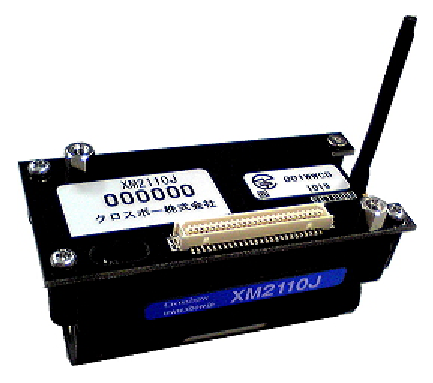
\includegraphics[width=40mm]{./images/iris_mote.eps}
    \end{center}
    \caption{Iris Mote}
    \label{fig:iris_mote}
 \end{minipage}
 \begin{minipage}{0.5\hsize}
    \begin{center}
     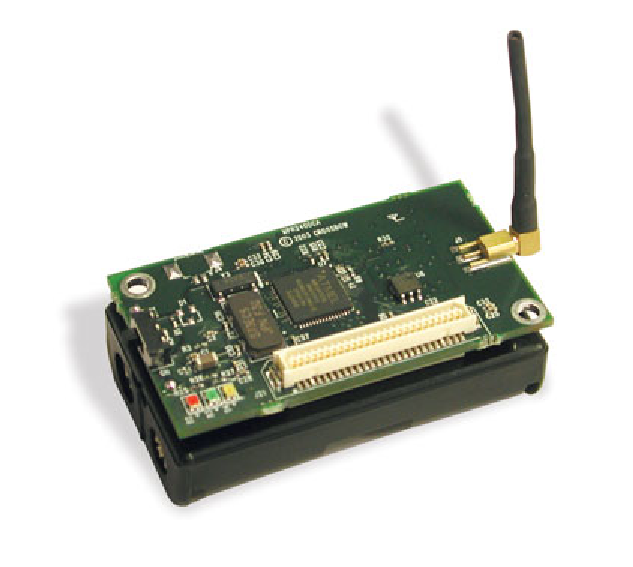
\includegraphics[width=45mm]{./images/micaz.eps}
    \end{center}
    \caption{MicaZ}
    \label{fig:micaz}
 \end{minipage}
\end{figure}

\begin{figure}[htbp]
 \begin{center}
  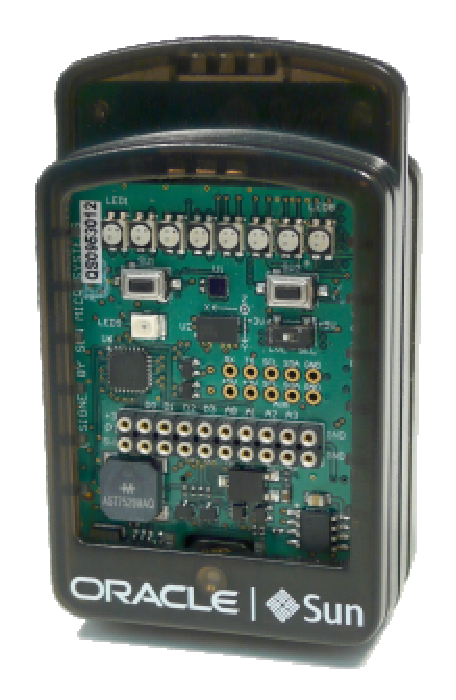
\includegraphics[width=25mm]{./images/sunspot.eps}
 \end{center}
 \caption{SunSPOT}
 \label{fig:sunspot}
\end{figure}





\section{環境モニタリング}

\subsubsection{森林火災検知}

\vspace{0.5em}センサノードが戦略的に,ランダムに,密集して森林に配置されれば,
火災が制御できなくなるほど広がる前に,
センサノードが正確な火の根源をユーザに知らせることが可能になる.
%Since sensor nodes may be strategically,randomly,and densely deployed in a forest,
%sensor nodes can relay the exact origin of the fire to the end users 
%before the fire is spread uncontrollable. 
数百万から構成されるセンサノードが
無線周波数を利用し,統合され,配置されることも可能である.
%Millions of sensor nodes can be deployed and integrated using radio frequencies/ optical systems. 
また,太陽電池などのような,利用可能なエネルギーを探索し,
効率的に活用する手法が備えられるかもしれない.
%Also,they may be equipped with effective power scavenging methods [12],
%such as solar cells,
%because the sensors may be left unattended for months and even years. 
センサノードは,分散しセンシングをするまたは木や岩のような障害に打ち勝つために,
それぞれが協調するだろう.
%The sensor nodes will collaborate with each other to perform distributed 
%sensing and overcome obstacles,
%such as trees and rocks,
%that block wired sensors’ line of sight.


山火事の消火においては,類焼を予測するために
温湿度の変化を観測することが重要である.
これまでは消防士が測定器を持って位置時間ごとに測定を行っていたが,
この手法では消防司令所への報告に数分を要することに加え,
類焼する可能性のある危険な場所に消防士を向かわせなければならない.
山火事を消火する消防士を支援するシステムである,
FireWxNet\cite{conf/mobisys/HartungHSH06}ではこのような温湿度の測定を,
無線センサネットワークとそのネットワーク間を
接続する長距離無線リンクで構成されるシステムを
利用して行うことを提案している(図\ref{fig:firewxnet_overview}).
実際にこのシステムを展開することで,
温湿度の測定結果や,データの通信成功率,バッテリ寿命について考察している.
局所的な測定をセンサネットワークで行い,
そのデータを長距離無線リンクで伝送することで,
より現実的な無線センサネットワークの展開ができるという結果を示している.

\begin{figure}[htbp]
 \begin{center}
  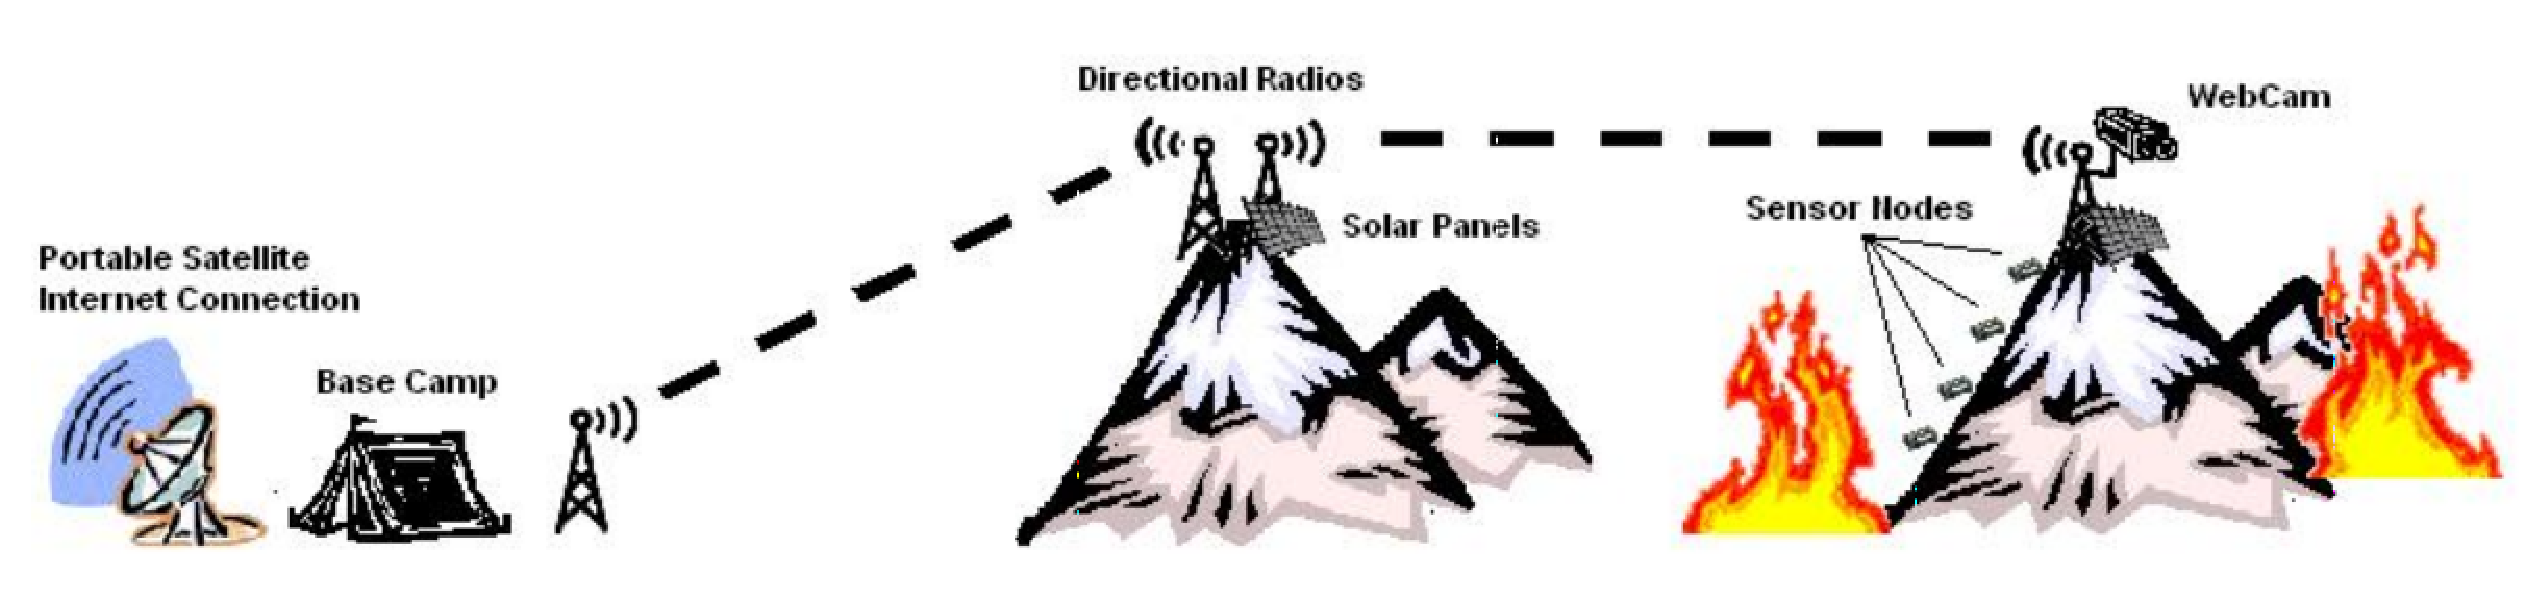
\includegraphics[width=140mm]{./images/firewxnet_overview.eps}
 \end{center}
 \caption{FireWxNet概要}
 \label{fig:firewxnet_overview}
\end{figure}


\section{ターゲットトラッキング}
%近年無線センサネットワークにおける,
%ターゲットトラッキングアプリケーション開発は
%ますます重要な位置づけになりつつある.
%Target Tracking as it moves through a sensor network has become an 
%increasingly important application in Wireless Sensor Networks. 

%物理環境において,
%特定のイベントの観測のための資源の限られた幾千ものセンサノードから成る,
%無線センサネットワーク技術に普及により,
%様々なシナリオにおける無線センサネットワークの利活用が
%現実的になりつつある.
%イベントを検知したセンサの周辺ノードはそのイベントを監視し,
%ラップトップやベースステーションのような外界と通信する機能を持った
%シンクノードに対してイベントの発生を知らせる.
%%The continuous evolution in wireless sensor network technology 
%%make it possible to implement the wireless sensor network (WSNs) in a variety of scenarios. 
%%WSNs consist of thousands of tiny sensor nodes deployed 
%%in a physical environment for observation of an event of interest. 
%%The sensors in the vicinity of an event must be able to monitor it and report back to the sink. 
%%A sink sensor node has capability to communicate with outside world such as laptop,base station. 
%
%
%近年,交通量管理や侵入者検知,野生動物の生態調査などの分野において,
%%センサノードは重要な役割を担っている.
%センサノードは重要な役割を担っている.
%無線センサネットワークにおける既存のターゲットトラッキングでは
%集約的な手法が用いられている.
%ネットワーク内におけるセンサの数が増加につれて,
%シンクノードに対するメッセージも増加し,
%それに伴い新たな帯域を消費してしまう.

%Sensor nodes have been deployed to play significant roles in traffic control,battlefield,
%habitat monitoring and intruder tracking in recent years. 
%The traditional target tracking methods for Wireless Sensor Networks 
%make use of a centralized approach. 
%As the number of sensors rise in the network,
%more messages are passed on towards the sink and will consume additional bandwidth. 
%Thus this approach is not fault tolerant 
%as there is single point of failure and lacks scalability. 
%Moreover in traditional target tracking methods,
%sensing task is usually performed by one node at a time resulting 
%in less accuracy and heavy computation burden on that node. 
%In WSNs each node has very limited power; 
%consequently traditional tracking methods 
%based on complex signal processing algorithms are not useful.

%物理環境において,
特定のイベントの観測のための資源の限られた幾千ものセンサノードから成る,
無線センサネットワーク技術に普及により,
様々なシナリオにおける無線センサネットワークの利活用が
現実的になりつつある.
特に交通量管理や侵入者検知,野生動物の生態調査などの
ターゲットトラッキングの分野において,
センサノードは重要な役割を担っており,
イベントを検知したセンサの周辺ノードはそのイベントを監視し,
ラップトップやベースステーションのような外界と通信する機能を持った
シンクノードに対してイベントの発生を知らせる.

ターゲットトラッキングにおいて,
対象を検知し,その旨をシステムのゲートウェイノードに警告するタスクにより
中継されたデータは,
適時にゲートウェイまで届けられるべきである.
このような時間的制約を伴ったデータの配送が必要なアプリケーションを想定した場合,
オペレーティングシステムとして
リアルタイム処理を行うことが可能なものを選択することが多い.
無線センサネットワークにおけるオペレーティングシステムのリアルタイム性については,
\ref{sec:threads_model}において詳細に述べる.
%ターゲットトラッキングアプリケーションにおいて,
%ある特定の時間にターゲットをセンシングしているセンサノードは
%アクティブモードを維持し,
%エネルギーを浪費しないように,
%残りのノードはターゲットが対象ノードに接近するまでの期間
%待機モードを継続する.
%この際,継続して移動するターゲットを監視するために,
%いくつかのセンサ郡は
%ターゲットが到着する少し前から
%アクティブモードにへと移行しなければならない.
%このアクティブなセンサ郡は
%移動するターゲットの速度に依存して変化し,
%クラスタのヘッドによってスケジューリングされる.
%ターゲットトラッキングを行う際には,
%エネルギーや帯域,オーバヘッドのような
%ネットワークリソース感のバランスを
%どのようにして保つかということに焦点が当てられている.
本節ではターゲットトラッキングの例として,
軍用監視システムと野生動物の生態調査について言及する.

%In a target tracking application,
%the sensor nodes which can sense the target at a particular time are kept in active mode 
%while the remaining nodes are to be retained in inactive mode 
%so as to conserve energy until the target approaches them. 
%To continuously monitor mobile target,
%a group of sensors must be turned in active mode just before target reaches to them. 
%This group of active sensors varies depending on the velocity of moving target and schedule from cluster head. 
%Ultimately, target tracking in course of maintaining the balance 
%between network resources like energy, bandwidth, and overheads is challenging.


%もし無線センサネットワークが適切に利用された場合,
%軍用のアプリケーションにおける情報収集にて,
%人間の力を必要とする機会が減少していき,
%近い将来には,
%センサデバイスが低価格で大量生産され,
%実社会に高密度に備え付けられることが予測される.

\subsubsection{軍用監視システム}

\vspace{0.5em}監視任務において,
ターゲットとする敵の能力や位置に関する情報を
正確に入手することが何よりも重要であるが,
そのような任務には隊員の危険を伴うものが多い.
無線センサネットワークを利用することで,
リスクを最小限に抑えつつ,
敵の侵入に関する情報を的確に把握する研究が盛んに行われている.
図\ref{fig:surveillance_system}は軍用監視システムにおける概念図である.

\begin{figure}[htbp]
 \begin{center}
  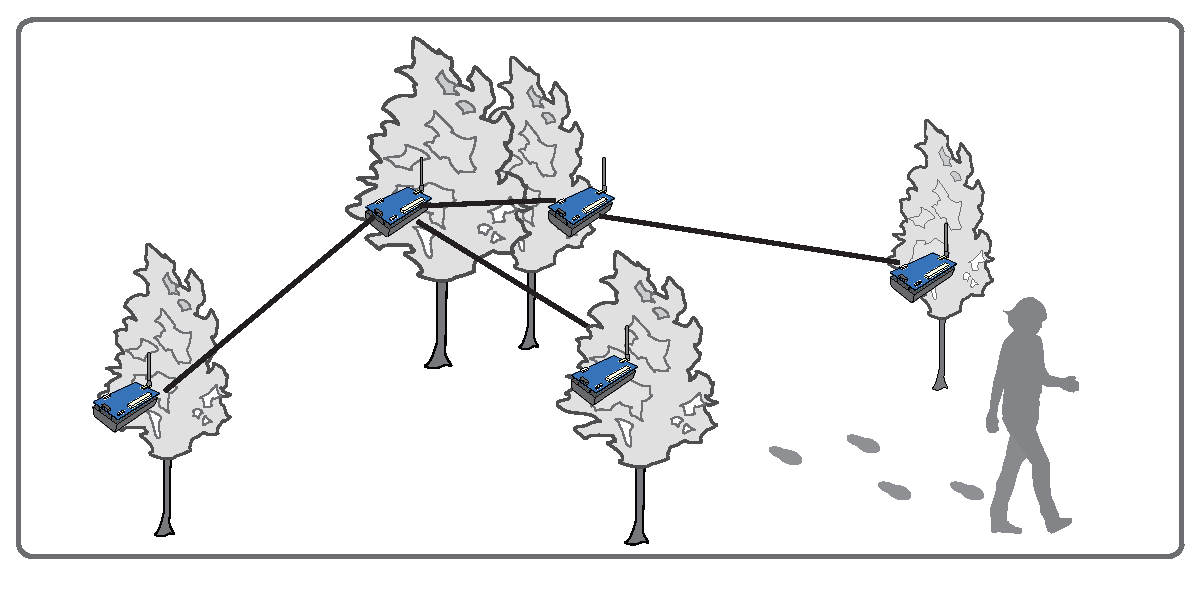
\includegraphics[width=100mm]{./images/surveillance_system.eps}
 \end{center}
 %\caption{イベント検知アプリケーション}
 %\caption{ターゲットトラッキングアプリケーション}
 \caption{軍用監視アプリケーションにおける概念図}
 \label{fig:surveillance_system}
\end{figure}


%監視アプリケーションにおいて,
%侵入者を検知し,その旨をシステムのゲートウェイノードに警告するタスクにより
%中継されたデータは,
%適時にゲートウェイまで届けられるべきである.
%上記のような時間的制約を伴ったデータの配送が必要なアプリケーションを想定した場合,
%オペレーティングシステムとして
%リアルタイム処理を行うことが可能なものを選択することが多い.
%無線センサネットワークにおけるオペレーティングシステムのリアルタイム性については,
%\ref{sec:threads_model}において詳細に述べる.

監視システムアプリケーションを用いた任務は
数日から数ヶ月にかけて行われるものが一般的であり,
任務中の秘密保持の重大性や
任務が敵の管轄地域行われる場合もあることから,
%近づきにくさ
任務期間中に資源の制限されたセンサデバイスの手動による充電はできないことがほとんどである.
したがって任務期間中継続して使用するために,
監視システムにおけるアプリケーションでは
センサデバイスの寿命を向上させるような
省エネルギーな構成が必要とされる.

また軍用の監視システムにおいて,
デイバイスが発見され,
それに伴い迎撃されることを
未然に防ぐことは極めて重要である.
センサデバイスを小型化することにより,
デバイスの発見を物理的に困難にすることができるが,
もしセンサデバイスが監視をする際に活発に通信をする場合,
無線周波数が傍受されてしまう可能性が高い.
重要なイベントが発生したときを除いて,
通信を控えることが求められている.

近年提案されている監視システムのほとんどが
シミュレーションを通して期待できる成果を挙げているが,
シミュレータを利用して単純化された仮説は
実環境において意図した通りの結果を得られないこともしばしばである.
Tian Heらの研究\cite{He04energy-efficientsurveillance}では,
省エネルギーかつステルス性を保ちながら移動する車両の位置を検知し,
追跡するセンサデバイスを用いた監視システムの設計と実装をし,
実空間においてシステムの感度を適宜調整することによって,
省エネルギー性と監視システムの性能におけるトレードオフについて考察している.
またこれに加えて,同期型の通信プロトコルを設計し,常にビーコンを送信し,
イベントが発生した場合はビーコンの送信を停止するProactive型と,
イベントが発生した場合にビーコンを送信するReactive型の実装を行い,
それぞれについて省電力性やステルス性などの評価も行っている.


\subsubsection{野生動物の生態調査}

\vspace{0.5em}



%\section{イベント検知アプリケーション}

\section{まとめ}
本章では,まず,公衆広域センサデータが多次元データであるということから,本研究の根幹を成す,Multidimensional Indexing(MI)という研究分野を紹介した.次に,Contents Delivery Network(CDN)という分散したデータセンターで多次元データを管理するネットワークという観点から捉え,センサデータにはCDNで扱われるような特殊性が存在しないことを述べた.最後に,公衆広域センサデータの分散管理手法を紹介し,センサデータの時間的特殊性が考慮されていないことに言及した.
